\documentclass[12pt,a4paper,notitlepage]{article}
\linespread{2.0}
\usepackage[T1]{fontenc}
\usepackage[utf8]{inputenc}
\usepackage{hyperref}
\usepackage{mathtools}
\usepackage{graphicx}

\begin{document}

\title{Technical Report on Convolutional Neural Networks}
\author{Sébastien Champoux 40133449
\\ ENGR 411 Technical Report
\\ Concordia University—Department of Computer Science
\\ Winter 2022
\\ Presented to Professor Nematollaah Shiri
}
\maketitle

\begin{abstract}
Convolutional neural networks (CNNs) are a class of artificial neural networks commonly used to analyze digital imagery. This report will discuss the structure, learning process and favourable characteristics of CNNs in the context of image classification.
\end{abstract}

\clearpage
\tableofcontents

\clearpage
\listoffigures

\clearpage

\section{Introduction}
Neural networks are one amongst many forms of machine learning. Convolutional neural networks are a specialized form of neural networks  that are especially well suited for image analysis applications, such as identifying and classifying objects within images. The following report will discuss different aspects of convolutional neural networks  in the context of image classification. Their structures, the deep learning process, image convolutions, pooling, and a discussion of favourable characteristics that make CNNs well suited for image classification.

\section{Multilayer Perceptrons}\label{fully-connected-networks}
Convolutional neural networks are enhanced versions of fully connected neural networks, also known as multilayer perceptrons. This first section will cover these simpler form of neural networks. The additional features of CNNs over multilayer perceptrons will be covered in section \ref{cnn-section}.

\subsection{Structure}
A common concrete application example for neural networks is the identification of handwritten digits. This application is commonly used as an example thanks to the existence of the MNIST Database (\textit{Modified National Institute of Standards and Technology database}), a database of 70,000 labelled pictures of handwritten digits freely available for machine learning \cite{lecun_mnist_1998}. To illustrate the presentation of multilayer perceptrons below, this application will be used to explain how the different components of a neural network can work together to achieve this application.

A multilayer perceptron is a class of neural network. As the name implies, it is made up of “neurons” that are connected together. A neuron is a real number in the range [0;1] that represents activation; 0.0 meaning the neuron is not activated and 1.0 meaning the neuron is fully activated. The neurons are arranged in multiple layers, at least three: an input layer, an output layer, and at least one “hidden” layer. The neurons in the input layer represent a part of the total input provided to the neural network. For our sample application, the input is a black and white image of a handwritten digit, of dimensions 28*28 pixels. Therefore, the input layer would contain 784 neurons, each corresponding to a pixel of the image. Their respective activation will be the brightness value of their respective pixel (0.0 being black, 1.0 being white, and shades of grey in between) \cite{sanderson_but_2017}.

The last layer represents the output of the neural network. As the perceptron performs image classification, each neuron in the output layer is one of the possible classifications of what could be represented in the image. For the digits example, the output layer would contain ten neurons, one for each digit. The intended output of the neural network is for one neuron to have a very high activation, and all the others to have a low activation. The activated neuron being the network's best guess of what digit is represented in the image \cite{sanderson_but_2017}.

The hidden layers, in between the input and output layers, serve to improve the performance of the neural network. These layers enable the network to recognize patterns within images, facilitating the recognition of complex shapes or objects. For instance, the digit “8” is made up of two small loops one over the other \cite{sanderson_but_2017}. Theoretically, the middle layers could attempt to recognize these shapes in the image to make a decision whether the digit represented is an eight. In practice, neural networks create their own patterns during the training process, which are often very abstract and far from what a human would consider logical \cite{sanderson_gradient_2017}.

Standard multilayer perceptrons are fully connected, meaning that every neuron from a layer is connected to every neuron from the previous layer. The activation of a neuron impacts the activation of every neuron connected to it in the following layer. Consequently, with the exception of neurons in the input layer, every neuron is a function of the activation of previous neurons in the network. The connection between two neurons can be weighted, to increase or decrease how much the activation of a neuron impacts the connection of another neuron \cite{sanderson_but_2017}.

\begin{figure}[htbp]
 \centering
  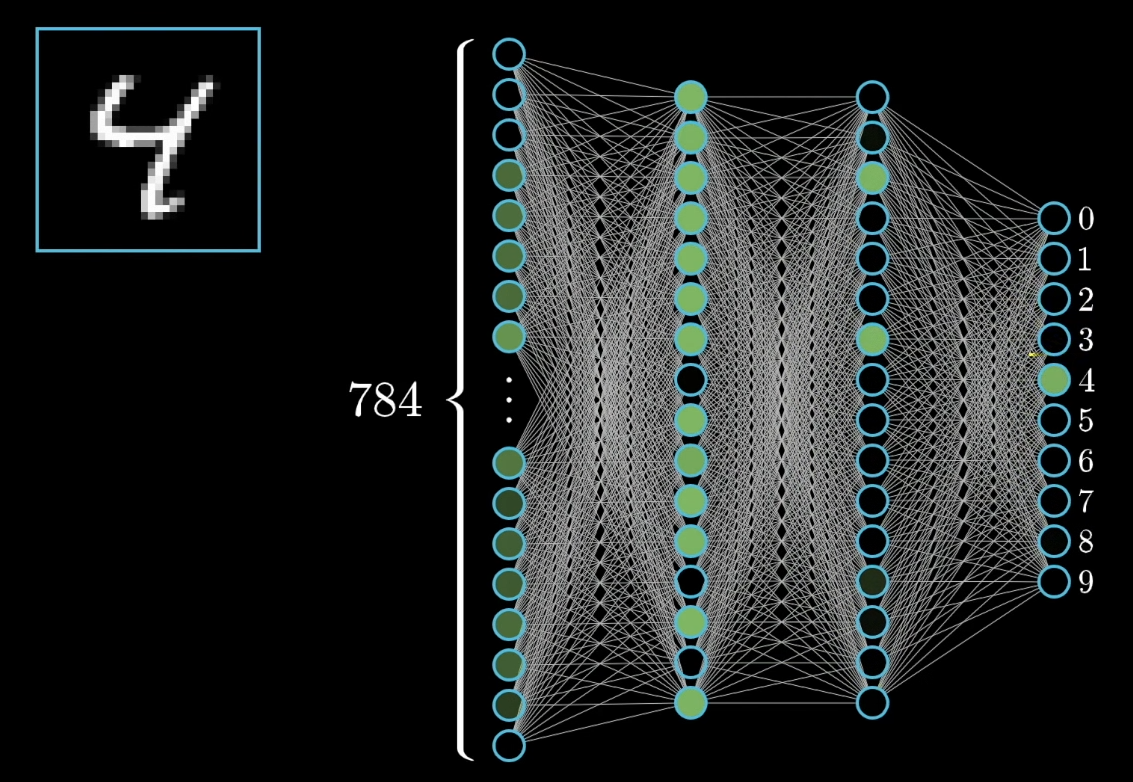
\includegraphics[width=0.60\textwidth]{images/perceptron-visualisation.png}
 \caption{Visualization of a multilayer perceptron \cite{sanderson_gradient_2017}}
 \label{fig:perceptron-visualisation}
\end{figure}

A bias can also be introduced to adjust further the connection between neurons. The addition of a bias can help improve the results by requiring a very high, or very low, activation from part of the input for neurons in the following layers to activate \cite{sanderson_but_2017}.

These elements can be summarized into a vector-matrix multiplication. Below is the equation to compute the activation of the neurons in hidden layer 1, based on the activation of neurons from the input layer (layer 0). \(a_i^{(0)}\) represents the activation of neuron \(i\) from layer 0. \(w_{i,j}\), the weight of the connection between neuron \(i\) from the input layer and neuron \(j\) in layer 1. \(b_i\), the bias applied to the weighted sum of the incoming connections from all neurons of layer 0 to neuron \(i\) in layer 1. This output vector is processed through the sigmoid function, to reduce the computed activations into the range \([0,1]\). The output vector represents the activation of every neuron in layer 1. This process can then be repeated for the subsequent layers, using the activation vector of layer 1 as input \cite{sanderson_but_2017}.

\begin{displaymath}
 \sigma
 \left(
 \begin{bmatrix}
  w_{0,0} & w_{0,1} & \cdots & w_{0,n}\\
  w_{1,0} & w_{1,1} & \cdots & w_{1,n}\\
  \vdots & \vdots & \ddots & \vdots\\
  w_{m,0} & w_{m,1} & \cdots & w_{m,n}
 \end{bmatrix}
 \begin{bmatrix}
  a_{0}^{(0)}\\
  a_{1}^{(0)}\\
  \vdots\\
  a_{n}^{(0)}
 \end{bmatrix}
 +
 \begin{bmatrix}
  b_{0}\\
  b_{1}\\
  \vdots\\
  b_{n}
 \end{bmatrix}
 \right)
 =
 \begin{bmatrix}
  a_{0}^{(1)}\\
  a_{1}^{(1)}\\
  \vdots\\
  a_{n}^{(1)}
 \end{bmatrix}
\end{displaymath}

As demonstrated above, a neural network boils down to a linear algebraic function. For this reason, neural networks are often computed by graphical processing units (GPUs) instead of regular CPUs, as GPUs are optimized for processing vector-matrix computations \cite{salter_cart_2021}.

\subsection{Deep Learning, Gradient Descent and Backpropagation}\label{deep-learning}

\subsubsection{Description of the process}
Once the structure of the neural network has been laid down, it must be fine-tuned to recognize and classify accurately what is presented to it. This tuning process consists of adjusting the hundreds of weights and biases that connect the neurons such that the neural network can classify its inputs with acceptable accuracy.

Given the large number of weights and biases, this is too tedious and intricate to be performed by humans. Therefore, the neural network “trains itself” thanks to two algorithms, gradient descent and backpropagation \cite{ibm_cloud_education_what_2020}.

To train a neural network, it is necessary to have a training set on hand. A training set is a set of content (images, videos, audio clips or some other medium), in which each item is labelled with the expected classification. As discussed earlier, the MNIST database is a good example of a training set: it is a set of 70,000 images of hand-drawn digits, each image appropriately labelled with the digit it contains \cite{lecun_mnist_1998}. Another example is the database created by Google's ReCAPTCHA service. This service helps to protect websites from bots by asking users to identify objects within images. By doing so, human users of ReCAPTCHA are also, unknowingly, contributing to the elaboration of training sets for AI deep learning \cite{maruzani_are_2021}.

To begin the training process, the different weights and biases of the neural network are initialized with random values. Then, the training set is processed by the neural network. After this first test, the results will be very poor. The network computes the accuracy (or lack thereof) of its results with a cost function. This function receives, as input, the different weights and biases in the neural network, and returns a real number, the average cost of the network's errors over the training set \cite{sanderson_gradient_2017}.

Below is the cost function of the neural network for one element of the training set. It is the sum of the squared difference between the activation of each neuron in the output layer (\(a_{j}^{(L)}\)) and their expected activation (\(y_{j}^{(L)}\)).

\begin{displaymath}
 C_{0}(w_{1,1}, w_{1,2}, ..., w_{i,j}, b_{1}, ... ,b_{j}) = \sum_{j=0}^{n_{L - 1}} (a_{j}^{(L)} - y_{j})^{2}
\end{displaymath}

This cost function expresses how accurate the results given by the neural network are. The higher the error cost, the greater the difference between the expected and computed results and thus, the less accurate the network. The objective is to adjust the weights and biases in the neural network to decrease this error cost as close as possible to zero over the training set \cite{sanderson_gradient_2017}.

To reduce this cost function, gradient descent will be used. Gradient descent is an optimization algorithm to find a local minimum in a function. The algorithm starts by computing the gradient of the cost function, noted \(\nabla C\): a vector towards the steepest increase for each weight and bias of the network. Then, the weights and biases are adjusted by a factor of \(-\nabla C\). Finally, these steps are repeated until a local minimum of the cost function is reached \cite{sanderson_gradient_2017}.

The algorithm to compute the gradient of a neural network  efficiently is backpropagation. For each element in the training set, the algorithm starts from the output layer, and compares the activations of the output layer's neurons to their expected ones. Then, it computes by how much each weight and bias that connects the output layer's neurons to the previous layer's neurons should be adjusted to minimize the error cost.  Connections (weights) that improve the accuracy of the results should be strengthened, and inversely, connections that worsen the results should see their weight diminished. Furthermore, these adjustments should be proportional to how much each connection impacts the error cost. This procedure is repeated recursively for each layer, from the output to the input layer. Finally, the adjustments computed for each example in the training set are averaged to get an adjustment vector for the entire training set. This algorithm is repeated multiple times until the neural network can process the training set with an acceptable level of accuracy \cite{sanderson_gradient_2017}.

Computing the gradient descent of a neural network over a very large training set is computationally expensive. For this reason, a more efficient technique, stochastic gradient descent, is commonly used. The algorithm is the same, but instead of computing the gradient vector for the entire training set, the training set is subdivided into smaller random subsets of training examples. Then, the gradient descent vector is computed for every subset of the training set, and these vectors are applied iteratively to improve the results of the network gradually \cite{sanderson_gradient_2017}.

\subsubsection{Calculus of deep learning}
The process described above is achieved using derivatives and the chain rule of calculus.

As a reminder of the notation, the equation below is the activation of a neuron that has not yet been processed through the sigmoid function (the weighted sum of the previous layer's neurons plus a bias). This weighted sum is represented as \(z_j^{(L)}\) to differentiate it from the activation of a neuron that has been reduced to [0;1] (represented as \(a_j^{(L)}\)). This equation is presented here separately from the activation function because it will be used to compute the 
cost function's gradient.

\begin{displaymath}
 z_j^{(L)} = w_{j0}^{(L)}a_0^{(L-1)} + w_{j1}^{(L)}a_1^{(L-1)} + \cdots + w_{jk}^{(L)}a_k^{(L-1)} + b_j^{(L)}
\end{displaymath}

Therefore, the activation for a neuron in the neural network can be represented as:
\begin{displaymath}
 a_j^{(L)} = \sigma\left(z_j^{(L)}\right)
\end{displaymath}

With these two equations established, it is now possible to compute how sensitive the cost function is to a change in a weight or bias. This can be computed with the derivative of the cost function over the derivative of a weight, thanks to the chain rule. The equation is represented below.
\begin{displaymath}
 \frac{\delta C_0}{\delta w_{jk}^{(L)}} =
 \frac{\delta z_j^{(L)}}{\delta w_{jk}^{(L)}}
 \frac{\delta a_j^{(L)}}{\delta z_j^{(L)}}
 \frac{\delta C_0}{\delta a_j^{(L)}}
 = a^{(L-1)} \sigma\prime(x^{(L)})((a^{(L)})^2)\prime
\end{displaymath}

Moreover, the formula above uses the derivative of the cost function over an activation (\(\frac{\delta C_0}{\delta a_j^{(L)}}\)). This derivative describes how sensitive the cost function is to a change in an activation. This is helpful to track ; it cannot be modified directly, but it is a result of changes to the weights and biases. To compute this derivative for neurons of the output layer, we use the output and expected activations. For neurons in the previous layers, we need to use the derivative of the cost function over the activation of previous layers. This is where the backpropagation algorithm gets its name from \cite{sanderson_backpropagation_2017}.
\begin{displaymath}
 \frac{\delta C_0}{\delta a_{k}^{(L-1)}} = 
 \sum_{j=0}^{n_{L} - 1}
 \frac{\delta z_j^{(L)}}{\delta a_{k}^{(L-1)}}
 \frac{\delta a_j^{(L)}}{\delta z_j^{(L)}}
 \frac{\delta C_0}{\delta a_j^{(L)}}
\end{displaymath}

The gradient descent vector is obtained by computing the derivative of the cost function over each weight and bias. Each component of this vector represents the adjustments that should be made to the different weights and biases in the neural network to minimize the cost function \cite{sanderson_backpropagation_2017}.
\begin{displaymath}
 -\nabla C =
 -\begin{bmatrix}
  \frac{\delta C_0}{\delta w_{0,0}^{(1)}}\\
  \frac{\delta C_0}{\delta w_{0,1}^{(1)}}\\
  \vdots\\
  \frac{\delta C_0}{\delta w_{j,k}^{(1)}}\\
  \frac{\delta C_0}{\delta b_{0}^{(1)}}\\
  \vdots\\
  \frac{\delta C_0}{\delta b_{k}^{(1)}}\\
 \end{bmatrix}
\end{displaymath}

\section{Convolutional and Pooling Layers}\label{cnn-section}
Convolutional neural networks are enhanced multilayer perceptrons that feature at least two additional, special purpose layers: a convolutional layer and a pooling layer. The image data is first processed through these two layers, and is subsequently flattened into an array to be fed to a regular perceptron for classification, as discussed in section \ref{fully-connected-networks} \cite{saha_comprehensive_2018}.

\begin{figure}[htbp]
 \centering
  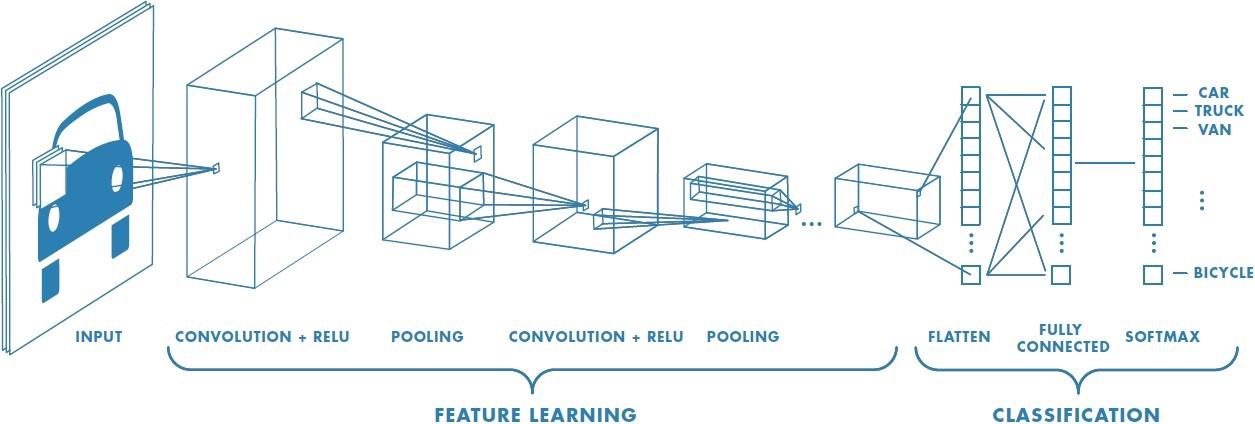
\includegraphics[width=0.70\textwidth]{images/convolutional-neural-network.jpeg}
 \caption{Illustration of a convolutional neural network \cite{saha_comprehensive_2018}.}
 \label{fig:convolutional-neural-network}
\end{figure}
\subsection{Image convolutions}

Image convolutions is a technique of image processing to create different effects in images, such as blurring, sharpening or highlighting edges. It consists of applying a kernel (a small square matrix) over the image, by computing the weighted average of the values of each pixel and its neighbours, according to the dimensions and weights of the kernel. \cite{sanderson_convolutions_2020}.
\begin{displaymath}
 \begin{bmatrix}
  1/9 & 1/9 & 1/9 \\
  1/9 & 1/9 & 1/9 \\
  1/9 & 1/9 & 1/9
 \end{bmatrix}
\end{displaymath}
\begin{figure}[htbp]
 \centering
  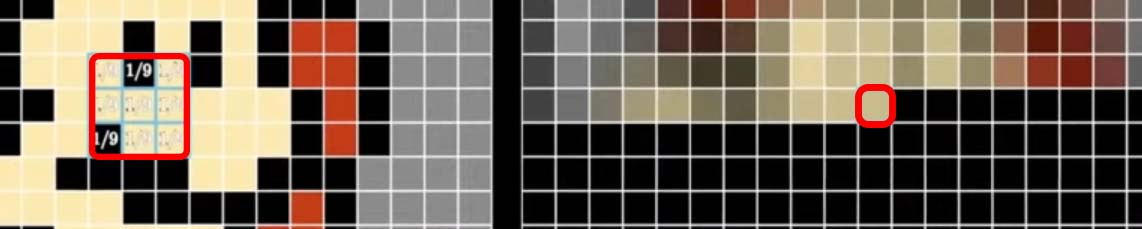
\includegraphics[width=1.00\textwidth]{images/box-blur.jpg}
 \caption{A group of beige and black pixels are averaged to a single grey-beige pixel by the box blur kernel \cite{sanderson_convolutions_2020}.}
 \label{fig:box-blur}
\end{figure}

As a simple example, the kernel above would create a box blur effect. For each group of nine pixels in the original image, the corresponding centre pixel in the blurred image would be equal to an average of the nine pixels, all with equal weights.

Another example of a possible simple kernel is \(\begin{bsmallmatrix}-1 & -1 & -1 \\ 1 & 1 & 1 \\ 0 & 0 & 0\end{bsmallmatrix}\). This kernel would highlight top edges of objects in an image \cite{deep_lizard_convolutional_2017}.
\begin{figure}[htbp]
 \centering
  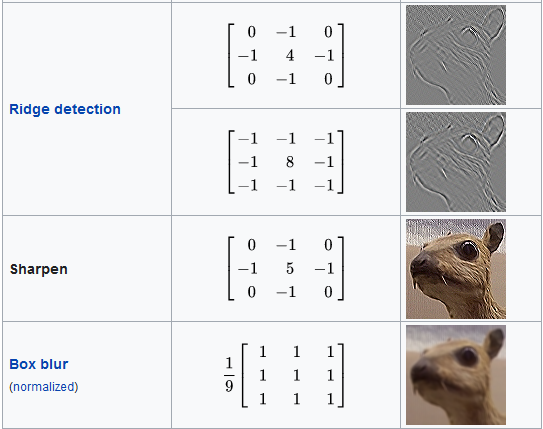
\includegraphics[width=0.8\textwidth]{images/image-convolutions-examples.png}
 \caption{Examples of kernels and their application on a sample image \cite{wikipedia_collaborators_kernel_2022}}
 \label{fig:image-convolutions-examples}
\end{figure}

An issue arises when the kernel is applied to pixels close to the edges. As each kernel of \(n^2\) pixels renders a single pixel in the image convolution, there will be a discrepancy between the original and convoluted image when the kernel is applied near the edges. Two techniques are used to deal with this situation: \textbf{valid padding} and \textbf{same padding}. For valid padding, the original image is padded with additional blank pixels beyond the edges. Consequently, the convoluted image has the same dimensions as the original image. For same padding, the original image is not padded, and the kernel is applied up to the image's edges only. This results in a convoluted image that is a few pixels smaller than its original \cite{sanderson_convolutions_2020}.
\begin{figure}[htbp]
 \centering
  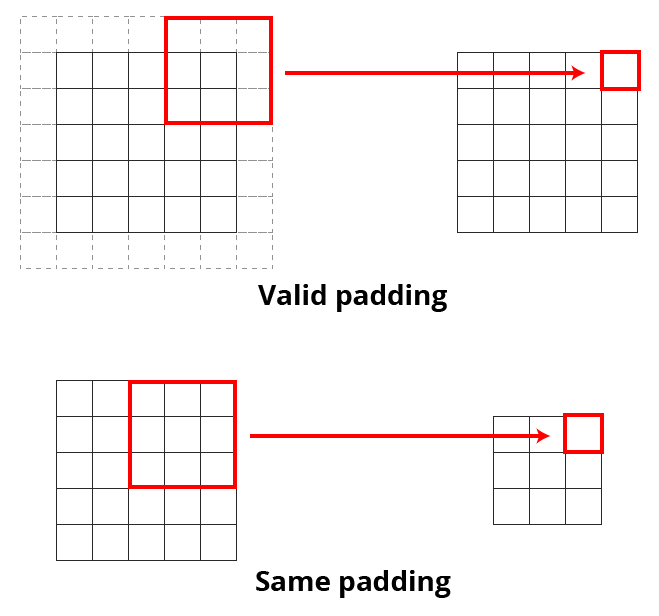
\includegraphics[width=0.80\textwidth]{images/padding-illustration.png}
 \caption{Comparison of same and valid padding algorithms (illustration by the author)}
 \label{fig:padding-illustration}
\end{figure}

\subsection{Convolutional layers}
The convolutional layers of a convolutional neural network apply image convolutions to the input images to extract additional information from them. The objective of the convolution operation is to extract high-level features from the input image, such as edges or corners. If multiple convolutional layers are used, conventionally, the additional layers will be responsible for detecting lower-level features, such as shapes or patterns. With enough layers, a convolutional neural network can 
acquire some very deep insight into the subject of an image \cite{saha_comprehensive_2018}.

The kernels used in the convolutional layers can be specified by the programmer. However, they can also be learned with backpropagation, as described in section \ref{deep-learning}, which is a strength of convolutional neural networks \cite{brownlee_gentle_2019}.

\subsection{Pooling layers}
The convolutional layers are very effective at highlighting features within an image, but they also have the downside of recording their precise location within the image frame. Therefore, transformations to the image, such as cropping, rotating or shifting will alter the feature map \cite{brownlee_gentle_2019}.
The most common solution to this problem is downsampling. Downsampling reduces the dimensions and resolution of an image. This results in a less detailed feature map, which preserves the large, important details, while foregoing the minor, less useful ones. This also diminishes the impact that the position, rotation or scale of an object has on the neural network's output \cite{brownlee_gentle_2019}.

One technique to downsampling is to change the stride of the image convolution. This means that when a kernel is convoluted over an image, instead of applying the kernel to every pixel, the kernel is only applied to every \(n^{th}\) pixel. Consequently, the convoluted image will contain only \(1/n\) of the pixels of the original image \cite{brownlee_gentle_2019}.

A more robust approach is to use a pooling layer. This layer applies a pooling operation to every feature map produced by the convolutional layer that preceeds it. For every group of \(n^2\) pixels in an image, a function is applied to reduce the pixel group to a single value. The size of the pooling operation is most often 2 * 2, which means that every image dimension will be reduced by half, and the number of pixels in the image will be reduced by a factor of four \cite{brownlee_gentle_2019}.

There are two common pooling algorithms: \textbf{max pooling} and \textbf{average pooling}. Max pooling returns the maximum value from each group of \(n^2\) pixels. 
Average pooling returns the average of the \(n^2\) pixels' values. Max pooling is generally preferred because, besides reducing the image's dimensions, it also discards unusual, noisy activations from the data, whereas average pooling does not discard noise \cite{saha_comprehensive_2018}.

\begin{figure}[htbp]
 \centering
  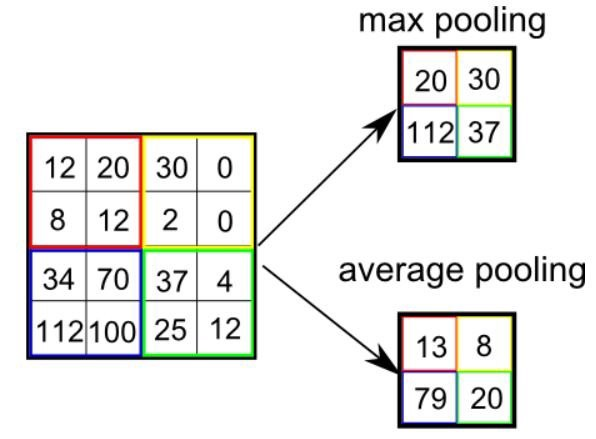
\includegraphics[width=0.80\textwidth]{images/pooling.jpg}
 \caption{Comparison of max and average pooling algorithms \cite{saha_comprehensive_2018}}
 \label{fig:pooling}
\end{figure}

Unlike convolutional layers, pooling layers are not machine-learned. They are always specified by the programmer \cite{brownlee_gentle_2019}.

\subsection{Image classification}
After processing the image through the convolutional and pooling layers, the processed image data is flattened into an array. This array is fed into a regular multilayer perceptron (fully connected layers), as discussed in section \ref{fully-connected-networks}. The classification is done via the soft-max classification algorithm. This is the technique described previously of the neural network returning a very high activation for the neuron that represents its best “guess” of the image's subject \cite{rosebrock_softmax_2016}.

\section{Favourable characteristics of CNNs for image classification}
Convolutional neural networks are frequently used to analyze visual imagery because they have several favourable characteristics over other classes of artificial intelligence that make them suitable for this purpose.

The use of convolutional layers preserves the spatial relationship of pixels. This is useful because in an image, a pixel is generally only relevant in the context of a few neighbouring pixels. These geometric relationships would be lost if the pixel data were flattened from the start. Furthermore, the neural network would be needlessly heavy if every pixel were analyzed in relation to every other pixel in the image. Therefore, the convolutional and pooling layers reduce the images to a form that is easier to analyze, without losing features that are critical for a good understanding of the image \cite{saha_comprehensive_2018}.

Since every pixel is analyzed only in relation to a few of its neighbouring pixels (within the range of a kernel), the first layers of a CNN do not need to be fully connected. This results in a neural network that is much lighter than a fully connected one, which improves performance. \cite{aghdam_guide_2017}

The use of multiple kernels in the convolutional layers improves the image analysis by enabling the detection of a large variety of details. Large-scale details such as edges or corners, and lower-scale details such as loops, can all be detected and fed into the algorithm to improve the accuracy of the image classification \cite{saha_comprehensive_2018}.

Finally, although the use of CNNs was only discussed in the context of image classification in this report, the possibilities of CNNs go way beyond that. For example, CNNs can detect multiple different objects within an image and identify their bounds to pixel precision, which could be very useful in photo editing softwares \cite{brownlee_gentle_2019}.

\section{Conclusion}
Convolutional neural networks are a class of neural networks commonly used to analyze digital imagery. They are made up of layers of “neurons” connected together by  weighted connections. Deep learning is the process used to tweak the thousands of weights and biases. Backpropagation is the algorithm that makes deep learning possible. It is performed by gradually increasing or decreasing the weights and biases to improve the network's accuracy over a representative training set. CNNs also feature convolutional layers, that aid in the detection of image features, and pooling layers, to remove variance and improve performance. This report discussed the use of CNNs in the context of image analysis, but more advanced applications, such as object identification, are also possible.

\clearpage
\begin{flushleft}
\bibliographystyle{plain}
\bibliography{references}
\end{flushleft}
\end{document}